\documentclass{article}
\usepackage{fullpage}
\usepackage{indentfirst}
\usepackage{amsmath}
\usepackage{amsfonts}
\usepackage{array}
\usepackage{tipa}
\usepackage{tikz}
\usepackage{tikz-qtree}
\usetikzlibrary{matrix, arrows, automata}
\usepackage{natbib}
\usepackage{gb4e}
\noautomath
\newcommand{\Y}{$\checkmark$}
\newcommand{\N}{\ding{55}}
\newcommand{\R}{$\Rightarrow$}
\newcommand\myeq{\mathrel{\stackrel{\makebox[0pt]{\mbox{\normalfont\tiny def}}}{=}}}
\newcommand{\ap}{\approx}
\title{Contour Spread in Zhenjiang}
\author{Chris Oakden}
\begin{document}
\maketitle
\citet{Bao1990}, citing \citet{Zhang1985}, presents evidence from Zhenjiang, a Mandarin dialect spoken in Jiangsu, as a case of contour spread. When any of a low-falling [31] (-u;hl), high-falling [42] (+u;hl) or `low'-rising [35] (-u;lh) appears before a high level tone [55] (+u;h), the [h] contour is said to spread regressively onto the preceding syllable, resulting in [22.55], [33.55], and [22.55] respectively. \textbf{add data points from Zhang here}.\footnote{Why /42/ becomes [33] and not [55] is the result of what Bao argues to be a domain-initial lowering rule. I will not go into the details here.} A graph of /31.55/$\mapsto$[22.55] is provided below:
\begin{center}
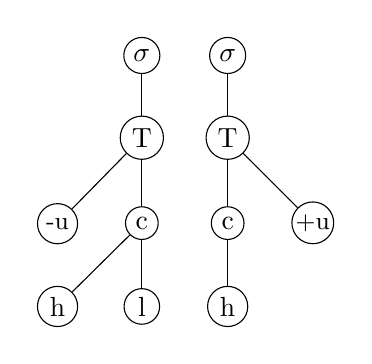
\begin{tikzpicture} [baseline = (y1.base)]
\matrix (m) [matrix of nodes, column sep = 1.5em, row sep = 1.5em]{
& \node[draw,circle, inner sep =2pt](x1){$\sigma$};  &  \node[draw,circle, inner sep =2pt](x2){$\sigma$};  \\
& \node[draw,circle, inner sep =2pt](y1){T}; &   \node[draw,circle, inner sep =2pt](y2){T}; \\
\node[draw,circle, inner sep =2pt](z1){\small -u}; & \node[draw,circle, inner sep =2pt](z2){c}; &   \node[draw,circle, inner sep =2pt](z3){c}; & \node[draw,circle, inner sep =.5pt](z4){\small +u}; \\
\node[draw,circle, inner sep =2pt](t1){h}; & \node[draw,circle, inner sep =2pt](t2){l}; &  \node[draw,circle, inner sep =2pt](t3){h}; & \\
};
\draw (x1) -- (y1);
\draw (x2) -- (y2);
\draw (z1) -- (y1);
\draw (z2) -- (y1);
\draw (z2) -- (t1);
\draw (z2) -- (t2);
\draw (y2) -- (z3);
\draw (y2) -- (z4);
\draw (z3) -- (t3);
\end{tikzpicture}
\hspace{.3cm}
$\rightarrow$
\hspace{.3cm}
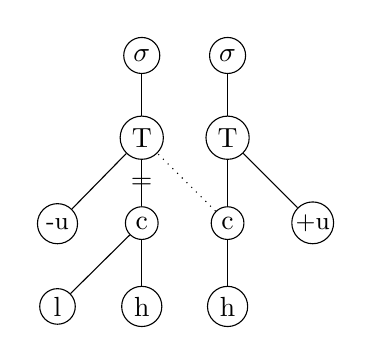
\begin{tikzpicture} [baseline = (y1.base)]
\matrix (m) [matrix of nodes, column sep = 1.5em, row sep = 1.5em]{
& \node[draw,circle, inner sep =2pt](x1){$\sigma$};  &  \node[draw,circle, inner sep =2pt](x2){$\sigma$};  \\
& \node[draw,circle, inner sep =2pt](y1){T}; &   \node[draw,circle, inner sep =2pt](y2){T}; \\
\node[draw,circle, inner sep =2pt](z1){\small -u}; & \node[draw,circle, inner sep =2pt](z2){c}; &   \node[draw,circle, inner sep =2pt](z3){c}; & \node[draw,circle, inner sep =.5pt](z4){\small +u}; \\
\node[draw,circle, inner sep =2pt](t1){l}; & \node[draw,circle, inner sep =2pt](t2){h}; &  \node[draw,circle, inner sep =2pt](t3){h}; &  \\
};
\draw (x1) -- (y1);
\draw (x2) -- (y2);
\draw (z1) -- (y1);
\path (z2) edge node{=} (y1);
\draw (z2) -- (t1);
\draw (z2) -- (t2);
\path (z3) edge (y2);
\draw (y2) -- (z4);
\draw (z3) -- (t3);
\draw [dotted] (z3) -- (y1);
\end{tikzpicture}
\hspace{.3cm}
$\rightarrow$
\hspace{.3cm}
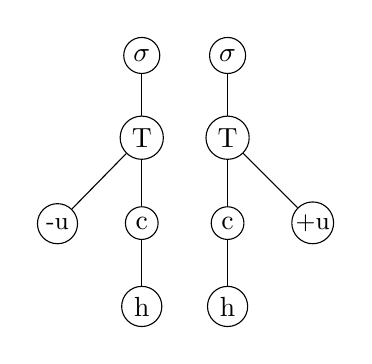
\begin{tikzpicture} [baseline = (y1.base)]
\matrix (m) [matrix of nodes, column sep = 1.5em, row sep = 1.5em]{
& \node[draw,circle, inner sep =2pt](x1){$\sigma$};  &  \node[draw,circle, inner sep =2pt](x2){$\sigma$};  \\
& \node[draw,circle, inner sep =2pt](y1){T}; &   \node[draw,circle, inner sep =2pt](y2){T}; \\
\node[draw,circle, inner sep =2pt](z1){\small -u}; & \node[draw,circle, inner sep =2pt](z2){c}; &   \node[draw,circle, inner sep =2pt](z3){c}; & \node[draw,circle, inner sep =.5pt](z4){\small +u}; \\
& \node[draw,circle, inner sep =2pt](t1){h}; &  \node[draw,circle, inner sep =2pt](t3){h}; &  \\
};
\draw (x1) -- (y1);
\draw (x2) -- (y2);
\draw (z1) -- (y1);
\draw (z2) -- (y1);
\draw (y2) -- (z3);
\draw (y2) -- (z4);
\draw (z3) -- (t3);
\draw (t1) -- (z2);
\end{tikzpicture}
\end{center}
In cases such as above, the `c' node on the second syllable spreads to the root node on the first syllable, causing the first `c' node to delink (and delete). As Bao explains, the `derived' structure post-spread is one in which each syllable contains an identical c-h complex (see especially discussion on p. 101). \par
Assuming this structure, we define a transduction from an input signature to an output signature to model regressive contour spread. Conflation of the spread contour node is represented as a \emph{copy} of the c-h complex from the final syllable attaching to the `T' node of the initial syllable. To do so, we define the transduction over a copy set of size 2, creating two copies of the portion of the structure that spreads (the `c' and `h' nodes in the final syllable).
\begin{equation}
\begin{aligned}
P_{\sigma}^{1}(x)&\myeq P_{\sigma}(x) & P_{\sigma}^{2}(x)&\myeq \mathtt{False} \\
P_{T}^{1}(x)&\myeq P_{T}(x) & P_{T}^{2}(x)&\myeq \mathtt{False}  \\
P_{+u}^{1}(x)&\myeq P_{+u}(x) & P_{+u}^{2}(x)&\myeq \mathtt{False} \\
P_{-u}^{1}(x)&\myeq P_{-u}(x) & P_{-u}^{2}(x)&\myeq \mathtt{False}  \\
P_{c}^{1}(x)&\myeq P_{c}(x) \land final(x) & P_{c}^{2}(x)&\myeq P_{c}(x)\land final(x) \\
P_{h}^{1}(x)&\myeq P_{h}(x) \land final(\delta(x)) & P_{h}^{2}(x)&\myeq P_{h}(x)\land final(\delta(x)) \\
P_{l}^{1}(x)&\myeq P_{l}(x) \land final(\delta(x)) & P_{l}^{2}(x)&\myeq P_{l}(x)\land final(\delta(x)) \\
\end{aligned}
\end{equation}
Unary relation definitions preserve only the `c' and terminal tonal nodes from the last syllable of the input structure, and generate an extra copy of that piece of structure in the second copy set. The remaining (and crucially the register) nodes are kept constant through the transduction. \par
Since association from TBUs to root nodes does not change, the association definition preserves input configuration. Other association possibilities---between copy sets or within the second copy set---are set to $\mathtt{False}$.
\begin{equation}
\begin{aligned}
\alpha^{1,1}(x)\ap y&\myeq\alpha(x)\ap y & \alpha^{1,2}(x)\ap y&\myeq\mathtt{False} \\
\alpha^{2,1}(x)\ap y&\myeq\mathtt{False} & \alpha^{2,2}(x)\ap y&\myeq\mathtt{False} \\
\end{aligned}
\end{equation} \par
Spread and conflation are the onus of the binary dominance function ($\delta(x)\ap y$). This definition achieves two goals: regressive `spread' of the final syllable's contour and maintenance of register features on both syllables.
\begin{equation}
\begin{aligned}
\delta^{1,1}(x)\ap y&\myeq \big[ P_{+u}(x)\land P_{T}(y)\land\delta(x)\ap y\big]\lor \\
&\quad \, \, \big[ P_{-u}(x)\land P_{T}(y)\land\delta(x)\ap y\big]\lor \\
&\quad \, \, \big[ P_{h}(x)\land P_{c}(y)\land final(\delta(x))\land final(y)\big]\lor \\
&\quad \, \, \big[ P_{l}(x)\land P_{c}(y)\land final(\delta(x))\land final(y)\big]\lor \\
&\quad \, \, \big[ P_{c}(x)\land P_{T}(y)\land final(x)\land final(y)\big]\lor \\
\delta^{1,1}(x)\ap y&\myeq\mathtt{False}\\
\delta^{2,1}(x)\ap y&\myeq P_{c}(x)\land P_{T}(y)\land final(x)\land penult(y) \\
\delta^{2,2}(x)\ap y&\myeq \big[ P_{h}(x)\land P_{c}(y)\land final(\delta(x))\land final(y)\big]\lor \\
&\quad \, \, \big[ P_{l}(x)\land P_{c}(y) \land final(\delta(x))\land final(y)\big] \\
\end{aligned}
\end{equation}
The first goal is achieved in the definition of domination within the first copy set, and between the second and first copy sets. The third, fourth, and fifth disjuncts of the $\delta^{1,1}(x)$ definition preserves c-T and t-c relations on the final syllable only. In the definition of $\delta^{2,1}(x)$, the copy of the final c-t complex is dominated by the tonal root on the first syllable of the first copy set, thus achieving spread (of the contour \emph{information}) and conflation (via a copy of `c' and terminal nodes \emph{distinct} from that which is dominated by the `T' node in the final syllable). The first and second disjuncts of $\delta^{1,1}(x)$ maintain input register features in the output structure (the second goal).\par
We establish linear order on the output structure by defining the successor function ($succ(x)\ap y$) as follows:
\begin{equation}
\begin{aligned}
succ^{1,1}(x)\ap y&\myeq \big[ P_{\sigma}(x)\land P_{\sigma}(y)\land succ(x)\ap y\big]\lor \\
&\quad \, \, \big[ P_{T}(x)\land P_{T}(y)\land succ(x)\ap y\big]\lor \\
&\quad \, \, \big[ P_{r}(x)\land P_{r}(y)\land succ(x)\ap y\big]\lor \\
&\quad \, \, \big[ P_{c}(x)\land P_{c}(y)\land final(x) \land final(y) \land succ(x)\ap y\big]\lor \\
&\quad \, \, \big[ P_{t}(x)\land P_{t}(y)\land final(\delta(x))\land final(\delta(y))\land succ(x)\ap y\big]\\
succ^{1,2}(x)\ap y&\myeq\mathtt{False} \\
succ^{2,1}(x)\ap y&\myeq \big[P_{c}(x) \land P_{c}(y) \land final(x) \land final(y)\land x\ap y\big] \lor \\
&\quad \, \, \big[P_{t}(x)\land P_{t}(y)\land final(\delta((x)) \land final(\delta(y))\land x\ap y\big] \\
succ^{2,2}(x)\ap y&\myeq \mathtt{False}
\end{aligned}
\end{equation}
The definition of the successor function above keep constant the ordering relations on syllable, `T' root, and register nodes, as well as the final `c' and terminal tonal nodes in the first copy set (recall that the final element in a tier is its own successor, and that the first c-t complex has been `deleted' from the structure. Since the copied `c' and `h' nodes in copy set 2 are elements of the first syllable, their successors will be their \emph{own equivalents} in the first copy set. The identity relation ($\ap$) isolates those specific structural positions in the definition of successor from the second copy set to the first. Therefore, the successor of the `c' node on the final syllable of the second copy of the input structure is the same position in the first copy set. The same is true for the terminal tonal node. Other possible ordering relations between or within copy sets is set to $\mathtt{False}$.  \par
Graphically, the transduction is:
\begin{center}
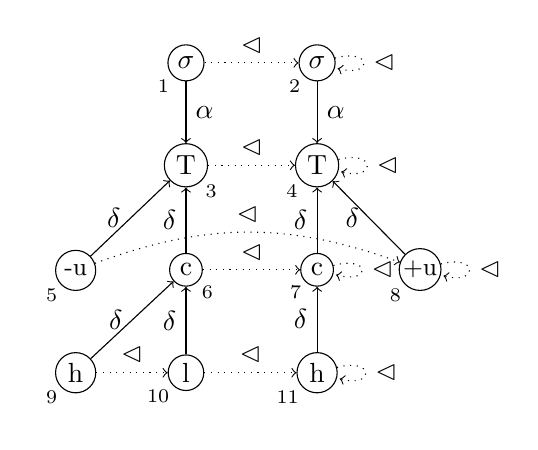
\begin{tikzpicture} [baseline = (y1.base)]
\matrix (m) [matrix of nodes, column sep = 1.5em, row sep = 1.5em]{
& \node[draw,circle, inner sep =2pt, label ={[label distance = -3pt] below left:\scriptsize1}](x1){$\sigma$};  &  \node[draw,circle, inner sep =2pt, label ={[label distance = -3pt] below left:\scriptsize2}](x2){$\sigma$};  \\
& \node[draw,circle, inner sep =2pt, label ={[label distance = -3pt] below right:\scriptsize3}](y1){T}; &   \node[draw,circle, inner sep =2pt, label ={[label distance = -3pt] below left:\scriptsize4}](y2){T}; \\
\node[draw,circle, inner sep =2pt, label ={[label distance = -3pt] below left:\scriptsize5}](z1){\small -u}; & \node[draw,circle, inner sep =2pt, label ={[label distance = -3pt] below right:\scriptsize6}](z2){c}; &   \node[draw,circle, inner sep =2pt, label ={[label distance = -3pt] below left:\scriptsize7}](z3){c}; & \node[draw,circle, inner sep =.5pt, label ={[label distance = -3pt] below left:\scriptsize8}](z4){\small +u}; \\
\node[draw,circle, inner sep =2pt, label ={[label distance = -3pt] below left:\scriptsize9}](t1){h};& \node[draw,circle, inner sep =2pt, label ={[label distance = -3pt] below left:\scriptsize10}](t2){l}; &  \node[draw,circle, inner sep =2pt, label ={[label distance = -3pt] below left:\scriptsize11}](t3){h}; &  \\
};
\draw [->] (x1) -- (y1) node[right, pos=.5]{$\alpha$};
\draw [->] (x2) -- (y2) node[right, pos=.5]{$\alpha$};
\draw [->] (z1) -- (y1) node[left, pos=.5]{$\delta$};
\draw [->] (z2) -- (y1) node[left, pos=.5]{$\delta$};
\draw [->] (z3) -- (y2) node[left, pos=.5]{$\delta$};
\draw [->] (z4) -- (y2) node[left, pos=.5]{$\delta$};
\draw [->] (t1) -- (z2) node[left, pos=.5]{$\delta$};
\draw [->] (t2) -- (z2) node[left, pos=.5]{$\delta$};
\draw [->] (t3) -- (z3) node[left, pos=.5]{$\delta$};
\draw [->, dotted] (x1) -- (x2) node[above,pos=.5]{$\vartriangleleft$};
\draw [->, dotted] (y1) -- (y2) node[above,pos=.5]{$\vartriangleleft$};
\draw [->, dotted] (z2) -- (z3) node[above,pos=.5]{$\vartriangleleft$};
\draw [->, dotted] (t1) -- (t2) node[above,pos=.5]{$\vartriangleleft$};
\draw [->, dotted] (t2) -- (t3) node[above,pos=.5]{$\vartriangleleft$};
\path [->, dotted] (z1) edge[bend left=20] node[above,pos=.5]{$\vartriangleleft$} (z4);
\path [->, dotted] (x2) edge[loop right] node{$\vartriangleleft$} (x2);
\path [->, dotted] (y2) edge[loop right] node{$\vartriangleleft$} (y2);
\path [->, dotted] (z3) edge[loop right] node{$\vartriangleleft$} (z3);
\path [->, dotted] (z4) edge[loop right] node{$\vartriangleleft$} (z4);
\path [->, dotted] (t3) edge[loop right] node{$\vartriangleleft$} (t3);
\end{tikzpicture}
\hspace{.5cm}
$\mapsto$
\hspace{.5cm}
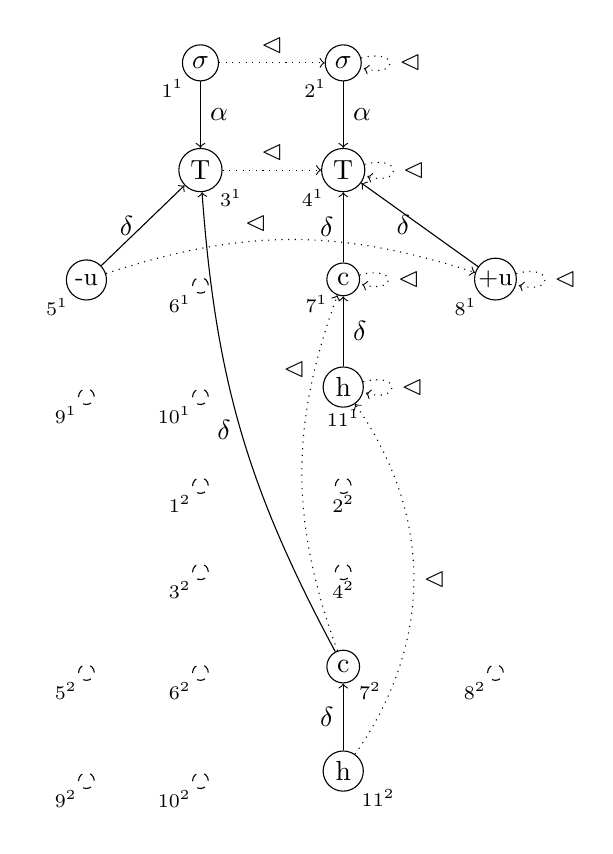
\begin{tikzpicture} [baseline = (y1.base)]
\matrix (m) [matrix of nodes, column sep = 1.5em, row sep = 1.5em]{
& \node[draw,circle, inner sep =2pt, label ={[label distance = -3pt] below left:\scriptsize$1^1$}](x1){$\sigma$};  &  \node[draw,circle, inner sep =2pt, label ={[label distance = -3pt] below left:\scriptsize$2^1$}](x2){$\sigma$};  \\
& \node[draw,circle, inner sep =2pt, label ={[label distance = -3pt] below right:\scriptsize$3^1$}](y1){T}; &   \node[draw,circle, inner sep =2pt, label ={[label distance = -3pt] below left:\scriptsize$4^1$}](y2){T}; \\
\node[draw,circle, inner sep =2pt, label ={[label distance = -3pt] below left:\scriptsize$5^1$}](z1){\small -u}; & \node[draw,circle, dashed, inner sep =2pt, label ={[label distance = -3pt] below left:\scriptsize$6^1$}](z2){\hspace{1em}}; &   \node[draw,circle, inner sep =2pt, label ={[label distance = -3pt] below left:\scriptsize$7^1$}](z3){c}; & \node[draw,circle, inner sep =.5pt, label ={[label distance = -3pt] below left:\scriptsize$8^1$}](z4){\small +u}; \\
\node[draw,circle, dashed, inner sep =2pt, label ={[label distance = -3pt] below left:\scriptsize$9^1$}](t1){\hspace{1em}};& \node[draw,circle, dashed, inner sep =2pt, label ={[label distance = -3pt] below left:\scriptsize$10^1$}](t2){\hspace{1em}}; &  \node[draw,circle, inner sep =2pt, label ={[label distance = -3pt] below:\scriptsize$11^1$}](t3){h}; &  \\
& \node[draw,circle, dashed, inner sep =2pt, label ={[label distance = -3pt] below left:\scriptsize$1^2$}]{\hspace{1em}}; & \node[draw,circle, dashed, inner sep =2pt, label ={[label distance = -3pt] below:\scriptsize$2^2$}]{\hspace{1em}}; \\
& \node[draw,circle, dashed, inner sep =2pt, label ={[label distance = -3pt] below left:\scriptsize$3^2$}]{\hspace{1em}}; & \node[draw,circle, dashed, inner sep =2pt, label ={[label distance = -3pt] below:\scriptsize$4^2$}]{\hspace{1em}}; \\
\node[draw,circle, dashed, inner sep =2pt, label ={[label distance = -3pt] below left:\scriptsize$5^2$}]{\hspace{1em}}; & \node[draw,circle, dashed, inner sep =2pt, label ={[label distance = -3pt] below left:\scriptsize$6^2$}]{\hspace{1em}}; & \node[draw,circle, inner sep =2pt, label ={[label distance = -3pt] below right:\scriptsize$7^2$}](z22){c};  & \node[draw,circle, dashed, inner sep =2pt, label ={[label distance = -3pt] below left:\scriptsize$8^2$}]{\hspace{1em}}; \\
\node[draw,circle, dashed, inner sep =2pt, label ={[label distance = -3pt] below left:\scriptsize$9^2$}]{\hspace{1em}}; & \node[draw,circle, dashed, inner sep =2pt, label ={[label distance = -3pt] below left:\scriptsize$10^2$}]{\hspace{1em}}; & \node[draw,circle, inner sep =2pt, label ={[label distance = -3pt] below right:\scriptsize$11^2$}](t22){h}; \\ 
};
\draw [->] (x1) -- (y1) node[right, pos=.5]{$\alpha$};
\draw [->] (x2) -- (y2) node[right, pos=.5]{$\alpha$};
\draw [->] (z1) -- (y1) node[left, pos=.5]{$\delta$};
\draw [->] (z3) -- (y2) node[left, pos=.5]{$\delta$};
\draw [->] (z4) -- (y2) node[left, pos=.5]{$\delta$};
\draw [->] (t3) -- (z3) node[right, pos=.5]{$\delta$};
\path [->] (z22) edge[bend left=12] node[left, pos=.5]{$\delta$} (y1);
\draw [->] (t22) -- (z22) node[left, pos=.5]{$\delta$};
\draw [->, dotted] (x1) -- (x2) node[above,pos=.5]{$\vartriangleleft$};
\draw [->, dotted] (y1) -- (y2) node[above,pos=.5]{$\vartriangleleft$};
\path [->, dotted] (z1) edge[bend left=18] node[above,pos=.4]{$\vartriangleleft$} (z4);
\path [->, dotted] (z22) edge [bend left=20]node[left,pos=.8]{$\vartriangleleft$} (z3);
\path [->, dotted] (t22) edge [bend right=35]node[right,pos=.5]{$\vartriangleleft$} (t3);
\path [->, dotted] (x2) edge[loop right] node{$\vartriangleleft$} (x2);
\path [->, dotted] (y2) edge[loop right] node{$\vartriangleleft$} (y2);
\path [->, dotted] (z3) edge[loop right] node{$\vartriangleleft$} (z3);
\path [->, dotted] (z4) edge[loop right] node{$\vartriangleleft$} (z4);
\path [->, dotted] (t3) edge[loop right] node{$\vartriangleleft$} (t3);
\end{tikzpicture}
\end{center}
\bibliographystyle{apalike}
\bibliography{references}
\end{document}